\hypertarget{P152}{}
\begin{solution}{normal} % 152
A heater with power $30\;\text{W}$ is designed for a mains voltage of $220\;\text{V}$. How large of a capacitor should be connected in series with the heater to reduce its power to $20\;\text{W}$? Do not consider the temperature-dependence of the heater's resistance into account.
\end{solution}

\hypertarget{P153}{}
\begin{solution}{normal} % 153
[IPhO 1982] A fluorescent lamp is connected to a mains electricity supply as shown in the figure below. The mains frequency is $50\;\text{Hz}$ and supplies an emf of $228.5\;\text{V}$. The current in the circuit is $0.60\;\text{A}$, the voltage across the lamp is $84\;\text{V}$, and the resistance in the coil is $26.3\;\Omega$. Assume that the fluorescent lamp is ohmic. Starter $S$ is a switch that closes when the lamp is switched on, but quickly opens again and remains open when the lamp is lit. a) What is the inductance $L$ of the coil? b) Determine the phase shift $\Delta\phi$ between the voltage and the current. c) What power $P$ is dissipated by the circuit? d) It is sometimes necessary to compensate for the reactive current resulting from the simultaneous use of many fluorescent lamps (see P154). A capacitor of what capacitance should be connected in series with the coil in order to reverse the phase shift? (Kalda Circuits P87)
\begin{center}
    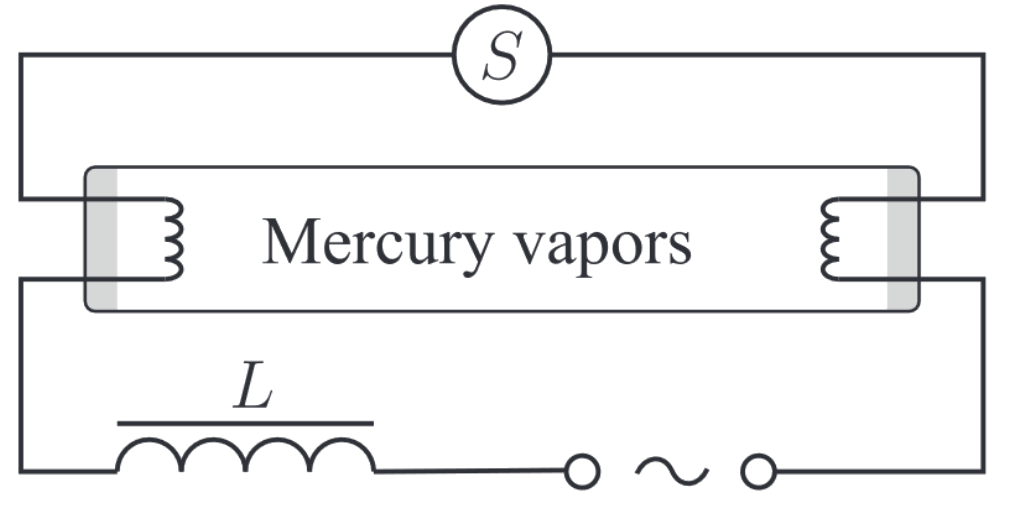
\includegraphics[width=0.65\textwidth]{S6 Figures/S6-153.png}
\end{center}
\end{solution}

\hypertarget{P154}{}
\begin{solution}{normal} % 154 ? actually have no idea what this is about
A cottage receives power from a substation via a long single-phase overhead power line. As a result, in addition to an electric meter, the house has a voltmeter to check the voltage reaching the house. After returning the the cottage after a three month absence, you discover that although all your appliances (including your lights) have been switched off, the transformer you were using had been consuming power. However, this energy consumption was not shown on your electric meter, and you want to determine how many kilowatt-hours of energy you didn't pay Eesti Energia for heating the air with an overhead line. To do this, you took three separate voltage readings: (1) $U_t=234.0\;\text{V}$ if only the transformer is connected to the mains; (2) $U_0=236.0\;\text{V}$ if everything (including the transformer) is switched off; and (3) $U_r=219.6\;\text{V}$ if the transformer is off but the electric radiator is on. You also determined, for the third case, that the power consumption of the radiator was $P_r=1200\;\text{W}$. Similarly, you recorded that if only the transformer is switched on, it consumes power $P_t=5\;\text{W}$. How many kilowatt-hours of energy did the transformer/overhead line consume during your absence?
\end{solution}

\hypertarget{P155}{}
\begin{solution}{normal} % 155
The figure below is also known as a Maxwell bridge, a circuit used to determine the inductance $L$ and resistance $R$ of the inductor. To do this, resistors $R_1,R_2,R_C$ and capacitor $C$ are adjusted until the voltmeter $V$ reads $0$. Determine $L$ and $R$ in terms of $R_1,R_2,R_C$, and $C$.
\begin{center}
    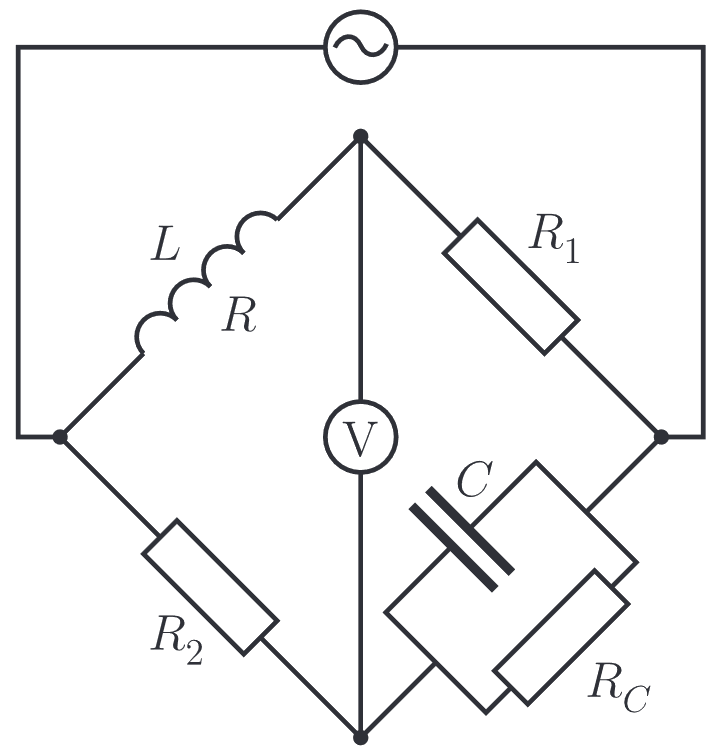
\includegraphics[width=0.5\textwidth]{S6 Figures/S6-155.png}
\end{center}
\end{solution}

\hypertarget{P156}{}
\begin{solution}{normal} % 156
The figure below shows a circuit that can be used to change the phase of an alternating signal. Show that, for a negligible output current, the output voltage is the same as the input voltage, but with a phase shift of $2\arctan(\omega RC)$ (or $2\arctan(-1/\omega RC)$). (Kalda Circuits P95)
\begin{center}
    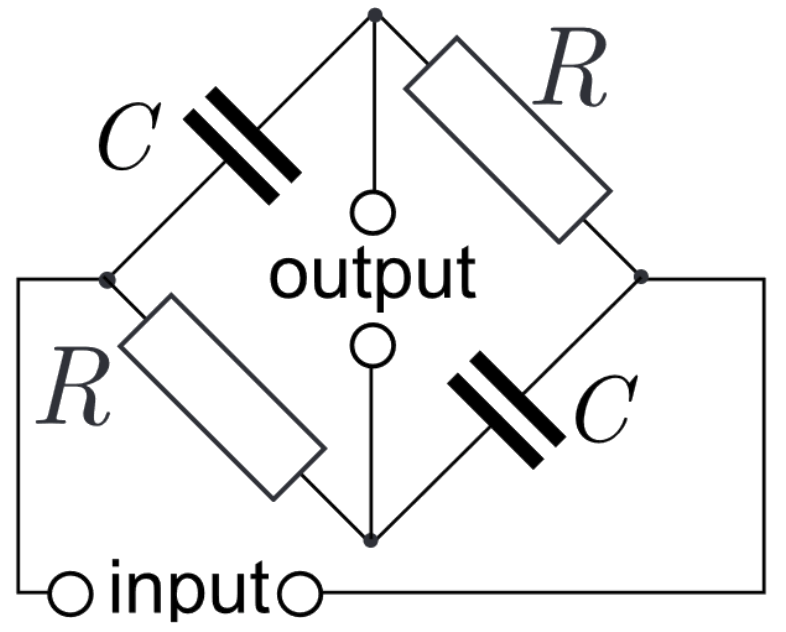
\includegraphics[width=0.45\textwidth]{S6 Figures/S6-156.png}
\end{center}
\end{solution}
\newpage
\hypertarget{P157}{}
\begin{solution}{normal} % 157
The circuit in the figure below is supplied with an AC voltage source with RMS voltage $U$. Determine the power dissipated in the circuit. \textit{Note:} The power dissipated can be found in two ways: by summing the individual powers $I^2R$ on all resistors or by using formula 9 for the whole circuit.
\begin{center}
    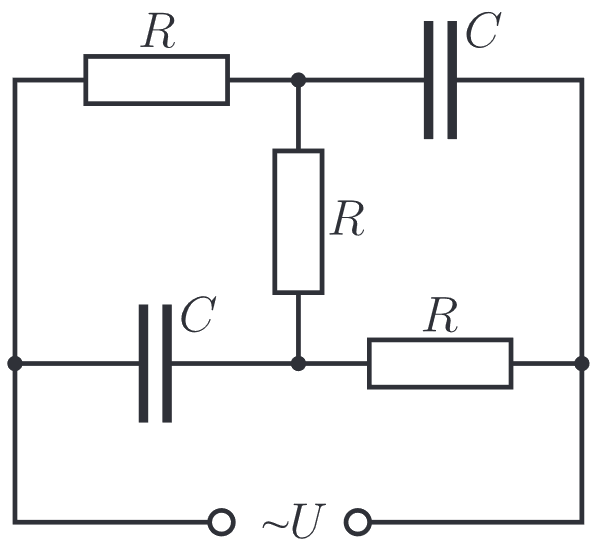
\includegraphics[width=0.35\textwidth]{S6 Figures/S6-157.png}
\end{center}
\end{solution}

\hypertarget{P158}{}
\begin{solution}{normal} % 158
The relationship between the voltages and currents of the primary and secondary coils of a transformer are generally very complex. However, real transformers are often close to an ideal transformer, which has the following properties: 1) The inductances $L_1$ and $L_2$ of the coils are very high; 2) The coupling between the primary and secondary coils is maximal; 3) The resistances of the coils are negligible; and 4) Losses in the core (hysteresis, eddy currents, etc.) are negligible. Show that in this case all currents and voltages have the same phase and the following equations hold:
$$\dfrac{U_2}{U_1}=n,\;\;\;\;\dfrac{I_2}{I_1}=\dfrac{1}{n},$$
where $n$ is the ratio between the number of turns in the secondary coil to the number of turns in the primary coil.
\end{solution}

\hypertarget{P159}{}
\begin{solution}{normal} % 159
In the LC circuit shown below, $L_1=10\;\text{mH}$, $L_2=20\;\text{mH}$, $C_1=10\;\text{nF}$, and $C_2=5\;\text{nF}$. At some point in time, the current through $L_1$ was equal to $I_1=0.1\;\text{A}$ and the voltage across $C_1$ at the same time was $U_0=40\;\text{V}$. What is the amplitude of current oscillations in coil $L_2$?
\begin{center}
    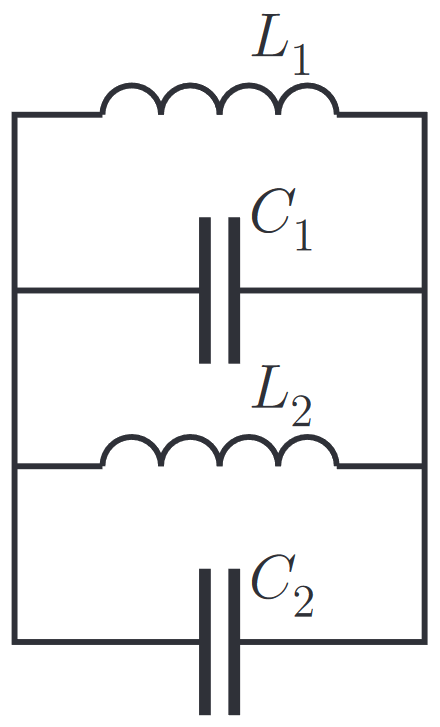
\includegraphics[width=0.22\textwidth]{S6 Figures/S6-159.png}
\end{center}
\end{solution}

\hypertarget{P160}{}
\begin{solution}{normal} % 160
Determine the natural oscillation frequency of the LC circuit shown below.
\begin{center}
    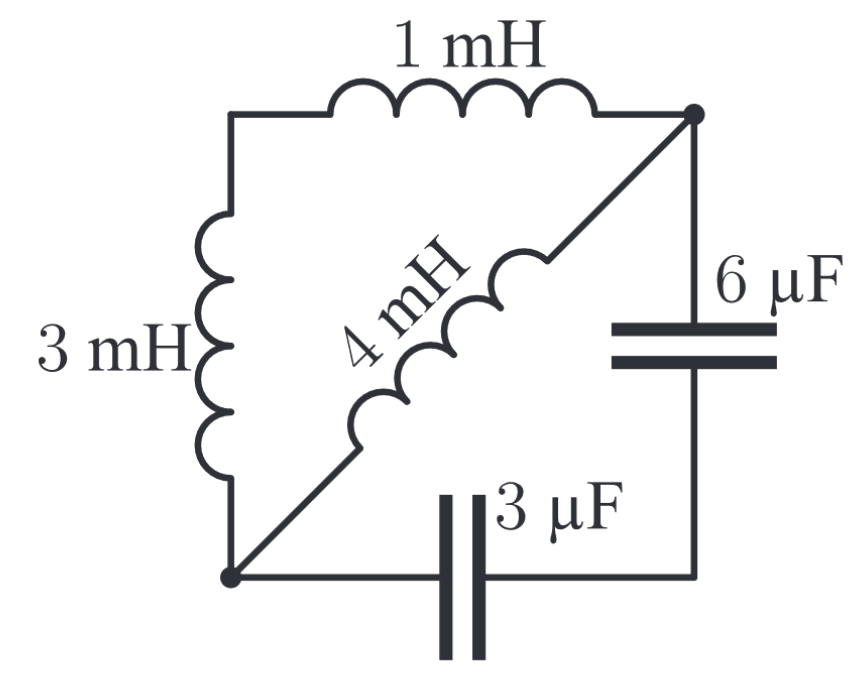
\includegraphics[width=0.4\textwidth]{S6 Figures/S6-160.png}
\end{center}
\end{solution}

\hypertarget{P161}{}
\begin{solution}{normal} % 161
Determine the natural oscillation frequencies of the LC circuit shown below. \textit{Note:} The equation $a^2=b^2$ satisfies both $a=b$ and $a=-b$. (Kalda Circuits P99)
\begin{center}
    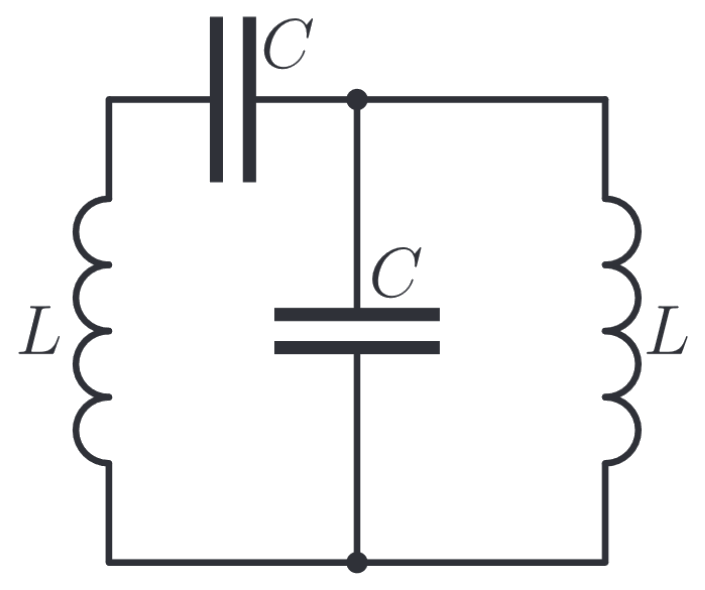
\includegraphics[width=0.4\textwidth]{S6 Figures/S6-161.png}
\end{center}
\end{solution}